\documentclass[10pt,letterpaper]{article}
\usepackage[utf8]{inputenc}
\usepackage{amsmath}
\usepackage{amsfonts}
\usepackage{amssymb}

\usepackage{hyperref}
\usepackage[usenames, dvipsnames]{color}
\usepackage{graphicx}
\usepackage{float}
\usepackage[T1]{fontenc}

\author{Michael Galliers \\ github \href{https://github.com/galliersm/CSC-310-Project-1}{https://github.com/galliersm/CSC-310-Project-1}}
\title{CSC 310 Project 1}
\date{October 26, 2018}
\begin{document}

\begin{titlepage}
\maketitle
\end{titlepage}

\paragraph{}
In this project we were tasked with creating Python programs to perform the
following operations: sorting a list using the Radix Sort algorithm and
evaluating a postfix (RPN) mathematical expression. Both of these algorithms
were to be implemented using data structures recently learned in our class:
queues and stacks.

\section{Radix Sort}

\begin{figure}[H]
\centering
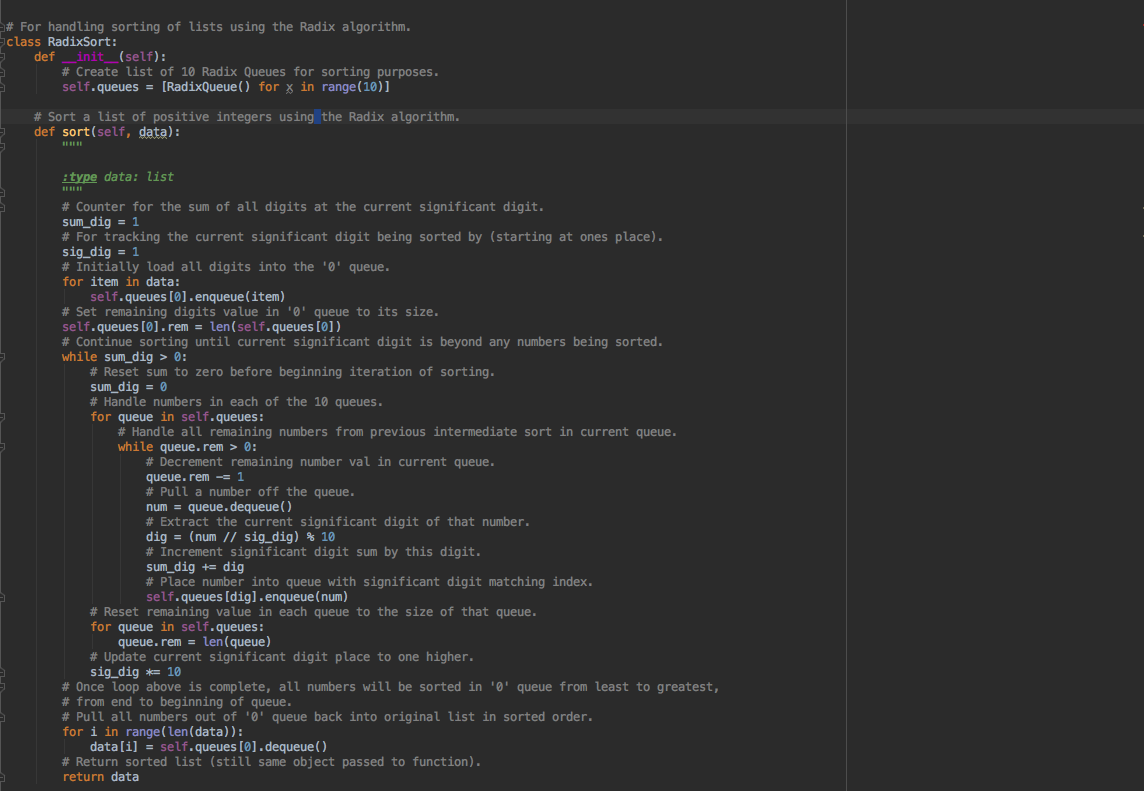
\includegraphics[width=\linewidth]{radix_sort_class.png}
\caption{Radix Sort Class}
\end{figure}

\paragraph{}
The Radix Sort algorithm is a counting based sorting algorithm. The algorithm
works by sorting positive integers one digit at a time, starting from the least
significant digit and moving on to the most significant digit. It does this by
extracting the current digit being sorted by from each number and then placing
the number in one of ten queues (indexed from 0 to 9) based on the value of
that digit. After this is complete, the numbers in each queue (processed from
queue 0 to queue 9) are sorted in the same way based on the next more
significant digit. This process continues until the digit being processed
exceeds the number(s) with the most digits. At this time, the queue of index 0
will have all the numbers sorted in non-decreasing order, such that the least
number will be the first to be dequeued.

\paragraph{}
The algorithm uses a modified queue ADT with an increased default capacity and
an extra attribute for monitoring the remaining numbers in the queue that need
to be processed. The sorting method itself is contained in the RadixSort class.
Upon instantiation, the class creates a list of 10 queues to be used for
sorting.

\paragraph{}
The sorting algorithm is contained in a method called “sort”. The method starts
out by creating counter-like variables for tracking when the sum of all digits
being analyzed is zero (i.e. the sorting is complete) and the specific digit
being analyzed. Initially, all numbers are loaded into the first queue
(index 0) and its remaining numbers variable is set to its size. Next, a loop
is run until the sum of all digits being analyzed is zero (i.e. sorting is
complete). The sum variable just mentioned is reset to 0 here before the digits
are processed. Then, it processes numbers in each of the ten queues, from
indices 0 to 9. While there are remaining numbers that need to be processed,
the method decreases the remaining number by 1, dequeues a number, extracts the
current digits being analyzed, increments the sum variable by this digit and
places the number in the queue having an index matching this digit. Since the
remaining variable of each queue tracks how many digits are in a queue from the
previous sorting, the numbers being enqueued during this sorting do not
interfere with the previous ones. After this sorting is complete, the remaining
variable of each queue is reset to its size and the digit being analyzed is
“incremented” to one digit more significant. After each sorting is complete,
each number is dequeued from the first queue and placed back into the list from
beginning to end. Then, the list object is returned. A simple user menu is
included for testing purposes. It takes a comma separated list of positive
integers, converts it to a list and returns the sorted result, asking if the
user would like to enter another list.

\begin{figure}[H]
\centering
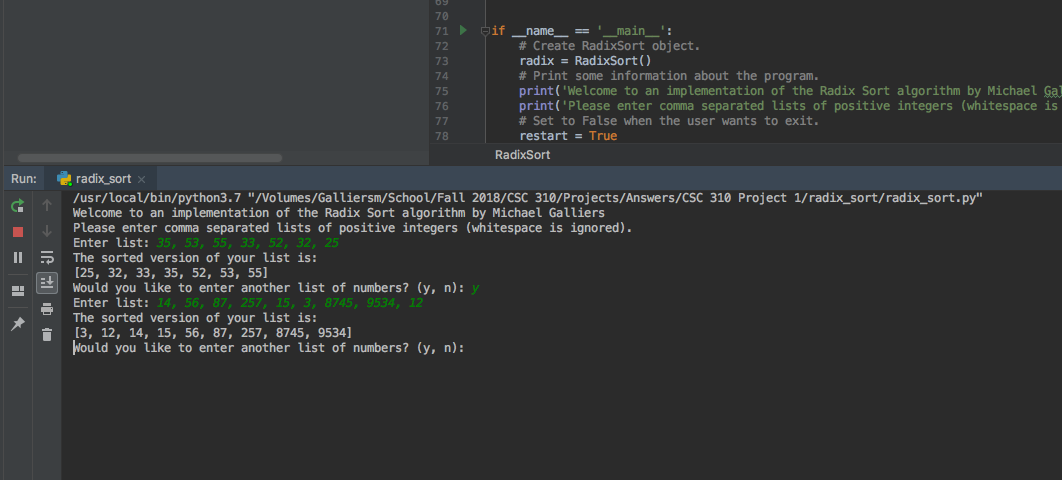
\includegraphics[width=\linewidth]{radix_sort_testing.png}
\caption{Radix Sort Testing}
\end{figure}

\section{Postfix}

\begin{figure}[H]
\centering
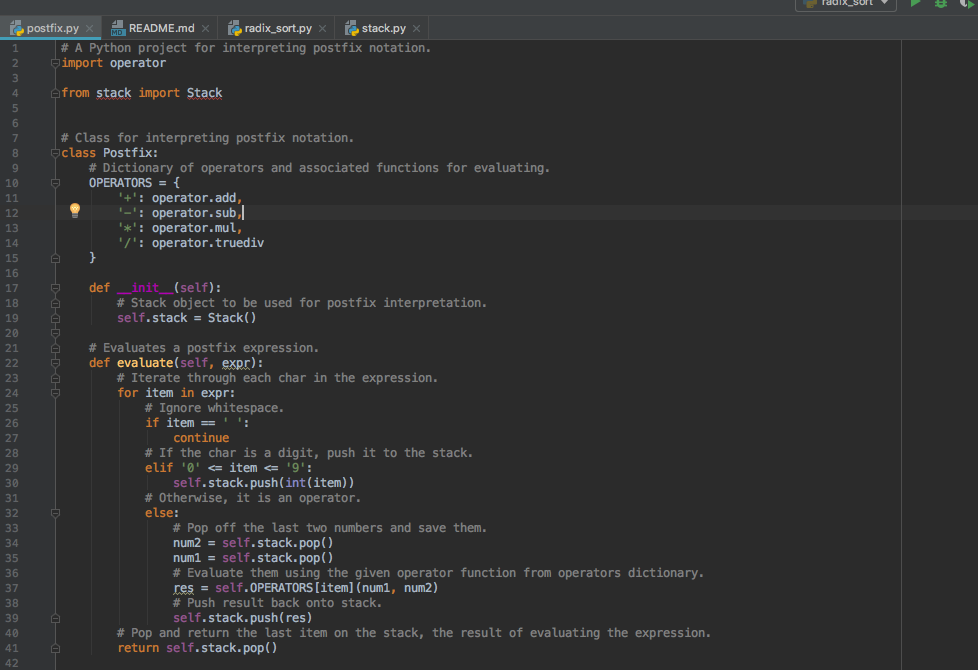
\includegraphics[width=\linewidth]{postfix_class.png}
\caption{Postfix Class}
\end{figure}

\paragraph{}
The postfix evaluator program is based on postfix notation (aka RPN). In this
notation, the operator is placed after the two numbers to be evaluated. Entire
mathematical expressions can be written this way making them much more
unambiguous than if traditional infix notation is used
(e.g. (7 + 2) * (4 / 2)). As a result, a simple stack-based algorithm can be
implemented to evaluate these expressions.

\paragraph{}
In the postfix program, a class is once again used to organize the components
of the algorithm. A dictionary of the valid operators as keys
(‘*’, ‘/’, ‘+’, ‘-‘) and imported “operator” functions that can evaluate each
operator as values is given to aid in the evaluation of these operators. Upon
instantiation, the class creates a stack to be used for evaluation throughout
the life of the object. The evaluate method is what does the actual
calculation. It takes a postfix expression as input. It then iterates through
each character of the expression. If it encounters a space, it is ignored. If
it finds a digit, it is type-casted to int datatype and pushed to the stack.
If an operator is encountered, the last two numbers are popped off the stack in
the order number2, number1 (due to design of stack) and saved to variables.
Then, using the aforementioned operator dictionary, the method for the operator
found is obtained and used to evaluate the numbers. Then, the result is pushed
back on the stack. After all the characters have been processed, the remaining
single number on the stack is the result, which is popped off and returned. A
simple user menu is included for testing purposes. It asks the user for a
postfix expression containing only valid operators and single-digit numbers and
prints the result. It then asks if the user would like to enter another number
or quit.

\begin{figure}[H]
\centering
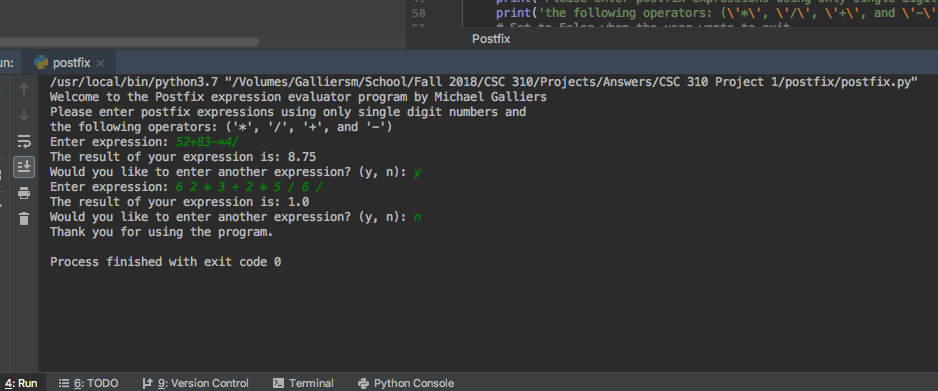
\includegraphics[width=\linewidth]{postfix_testing.png}
\caption{Postfix Testing}
\end{figure}

\section{Conclusion}
In conclusion, this project encouraged the students to apply concepts learned
in class to real life programming problems. Throughout computer science
training in college, it is important to remember that knowledge of concept is
only important if you know how to apply them. Otherwise, it is just head
knowledge. I learned a lot about how to apply the concepts we learned in class
in this assignment and am looking forward to the next programming project we
have.


\end{document}